\section{CSI300 rolling-residual prediction intervals}
\label{sec:intervals}
Point-loss improvements need not improve interval forecasts. This section applies the same absolute-residual construction to all five models and evaluates the 30 combinations of model, nominal coverage, and calibration window described in Section~\ref{sec:methods}. Width and interval score are reported on the log-target scale.

\subsection{A common evaluation sample}
DEC and XGB-AR do not have corrected predictions in the first-stage validation segment, so they first accumulate 60 realized test residuals. All settings are then evaluated on the same 1859 dates, from 2018-07-27 to 2026-03-30. Other models may still use their available validation residuals for calibration: common evaluation dates do not require discarding information that would already have been available to a model. All interval figures and coverage diagnostics use this same evaluation sample.

\begin{table}[htbp]\centering
\caption{Common-date 90\% intervals with calibration window 250.}
\label{tab:interval_main}\label{tab:common_intervals}
\begin{tabular}{lrrrr}\toprule Model & $N$ & Coverage & Mean width & Mean score\\\midrule
HAR & 1859 & 0.9005 & 6.9949 & 9.6973\\
GARCH(1,1) & 1859 & 0.8967 & 9.1225 & 12.6634\\
XGB-Market & 1859 & 0.8983 & 7.0644 & 9.8534\\
XGB-AR & 1859 & 0.9021 & 7.0662 & 9.8793\\
DEC & 1859 & 0.8989 & 7.0634 & 10.1995\\\bottomrule
\end{tabular}
\end{table}

DEC's interval score is worse than those of HAR, XGB-Market, and XGB-AR, although better than GARCH's under this construction. Its interval is slightly narrower than those of the two XGB comparators, but that small width advantage does not offset the score penalties for misses. No significance test of interval-score differences is reported. The GARCH comparison concerns the same log-residual interval algorithm, not intervals derived directly from the model's conditional innovation distribution.

\begin{figure}[htbp]\centering
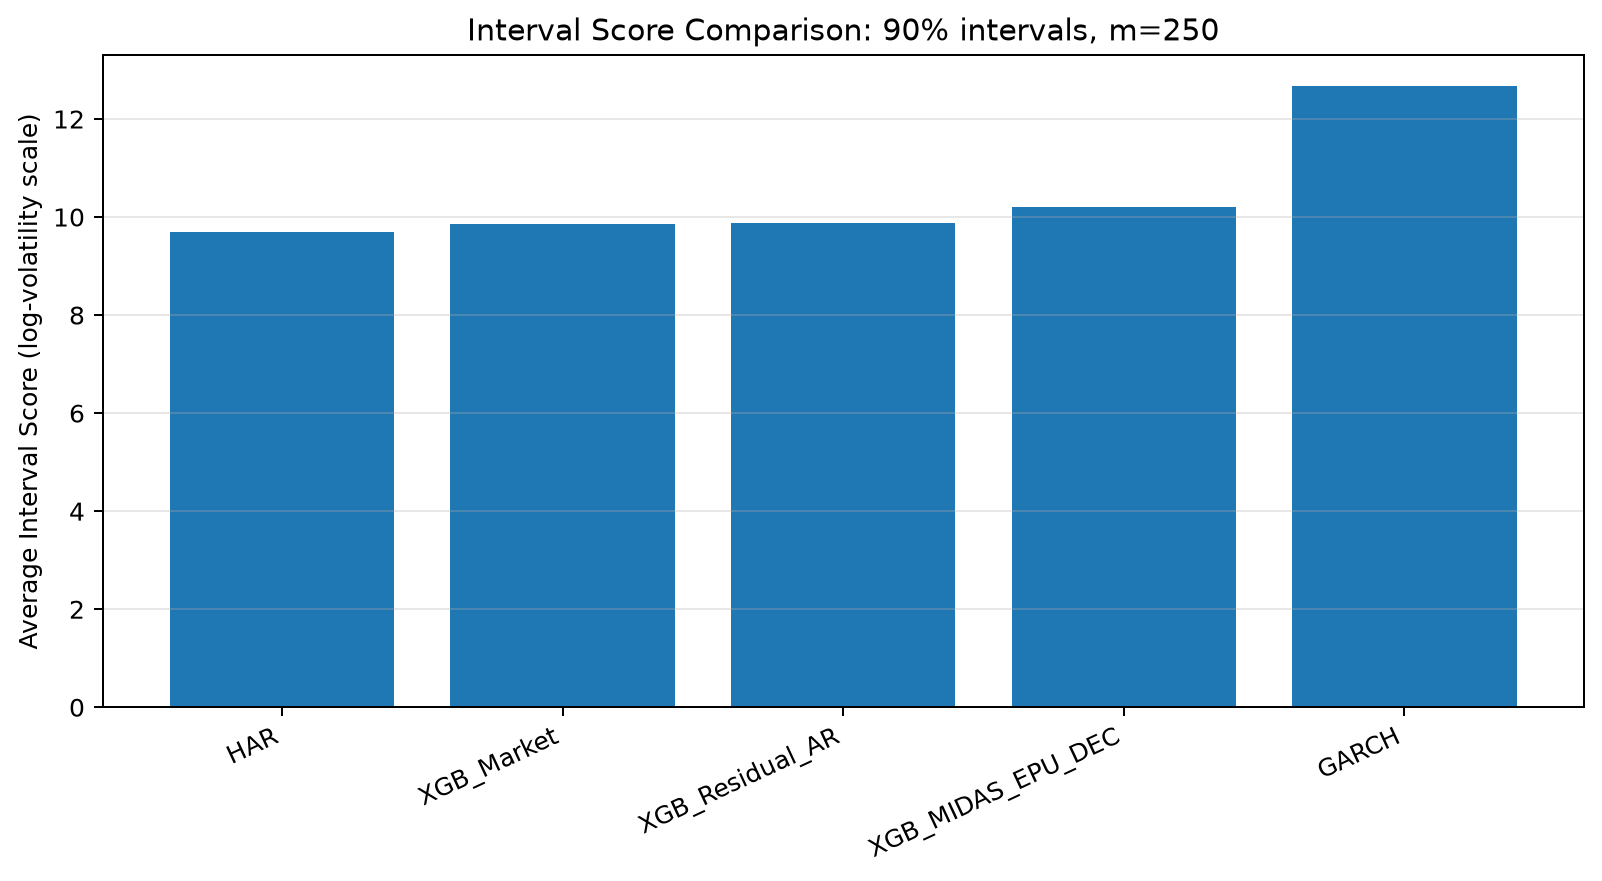
\includegraphics[width=.9\textwidth]{../../results/revised/intervals/fig_interval_score_main.png}
\caption{Mean interval scores on the common evaluation dates. Lower is better.}
\label{fig:interval_score_main}
\end{figure}
\begin{figure}[htbp]\centering
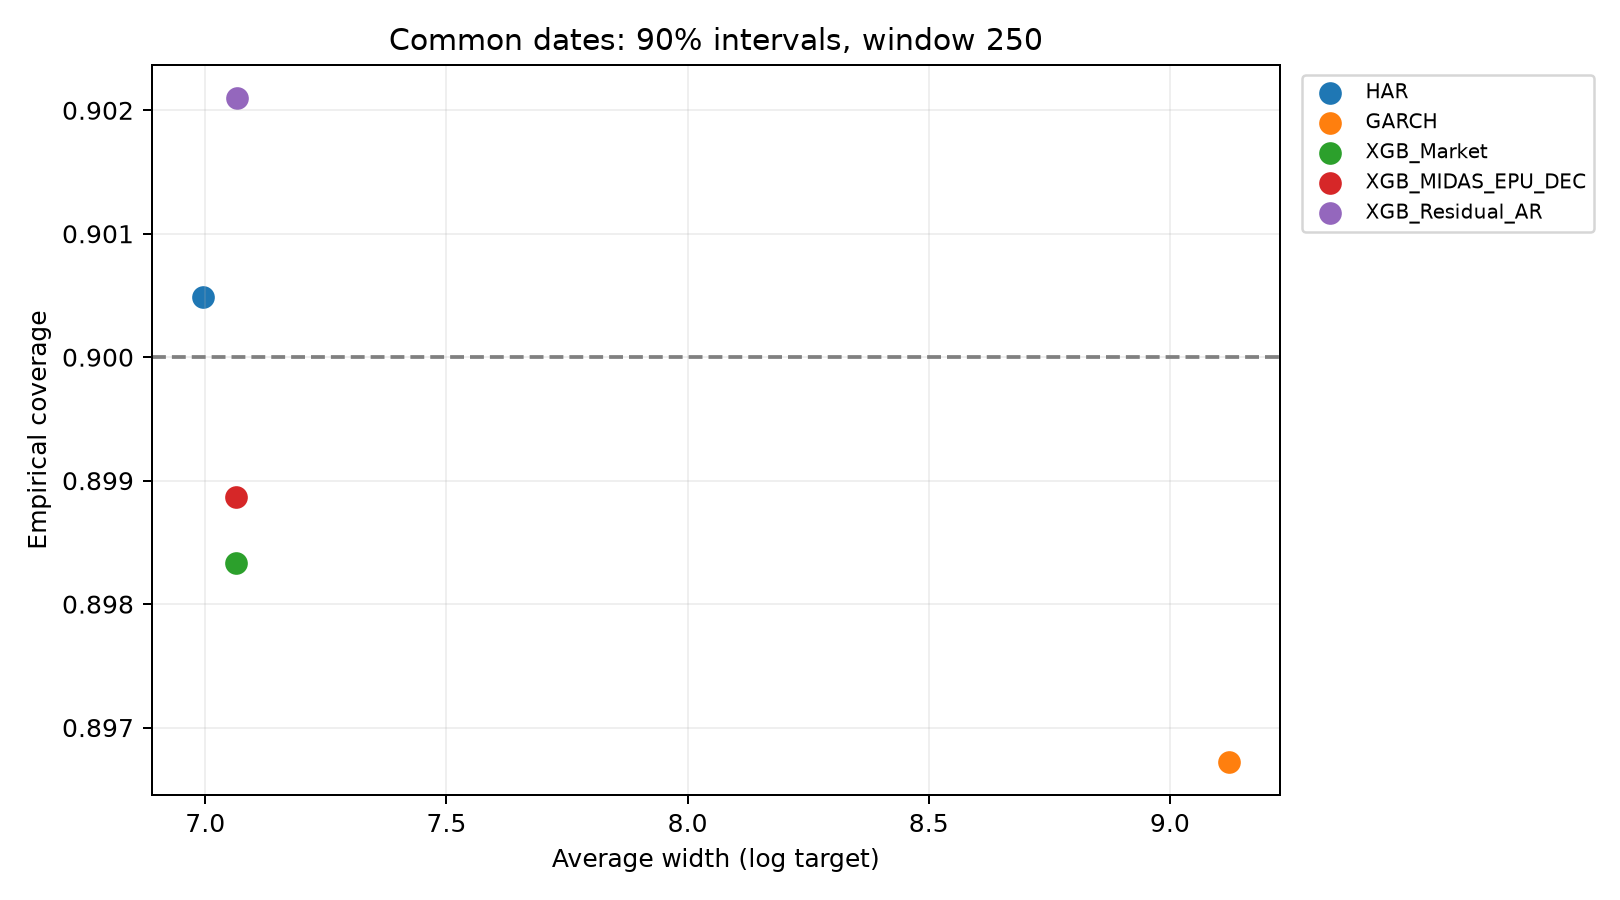
\includegraphics[width=.9\textwidth]{../../results/revised/intervals/fig_coverage_width_tradeoff_main.png}
\caption{Empirical coverage and mean width under the main setting.}
\label{fig:coverage_width_tradeoff}
\end{figure}

\subsection{Coverage diagnostics and temporal behavior}
Christoffersen-style diagnostics examine unconditional coverage (UC), independence of violations (IND), and joint conditional coverage (CC). For the main setting, none of the five models is rejected at the 5\% reference level (Table~\ref{tab:christoffersen_main}). Non-rejection is not proof of correct coverage, and these coverage diagnostics are not adjusted for multiple testing.

\begin{table}[htbp]\centering
\caption{Coverage diagnostics for the main common-date setting.}
\label{tab:christoffersen_main}
\begin{tabular}{lrrrr}\toprule Model & Violations & $p_{uc}$ & $p_{ind}$ & $p_{cc}$\\\midrule
HAR & 185 & 0.9445 & 0.1024 & 0.2629\\
GARCH(1,1) & 192 & 0.6388 & 0.1370 & 0.2964\\
XGB-Market & 189 & 0.8110 & 0.0987 & 0.2487\\
XGB-AR & 182 & 0.7623 & 0.1896 & 0.4041\\
DEC & 188 & 0.8712 & 0.0880 & 0.2303\\\bottomrule
\end{tabular}
\end{table}

The less favorable settings must also be retained. At 95\% nominal coverage with a window of 120, DEC has $p_{ind}=0.0062$ and $p_{cc}=0.0233$, indicating clustered violations under these reference diagnostics. A favorable aggregate coverage rate can conceal local failures.

Figure~\ref{fig:rolling_coverage} uses overlapping 60-observation windows; adjacent values are therefore not independent replications. The recent interval path in Figure~\ref{fig:interval_series_xgb_midas} is a descriptive view of sample behavior, not evidence that every miss is attributable to unforeseeable noise or a sudden shock.

\begin{figure}[htbp]\centering
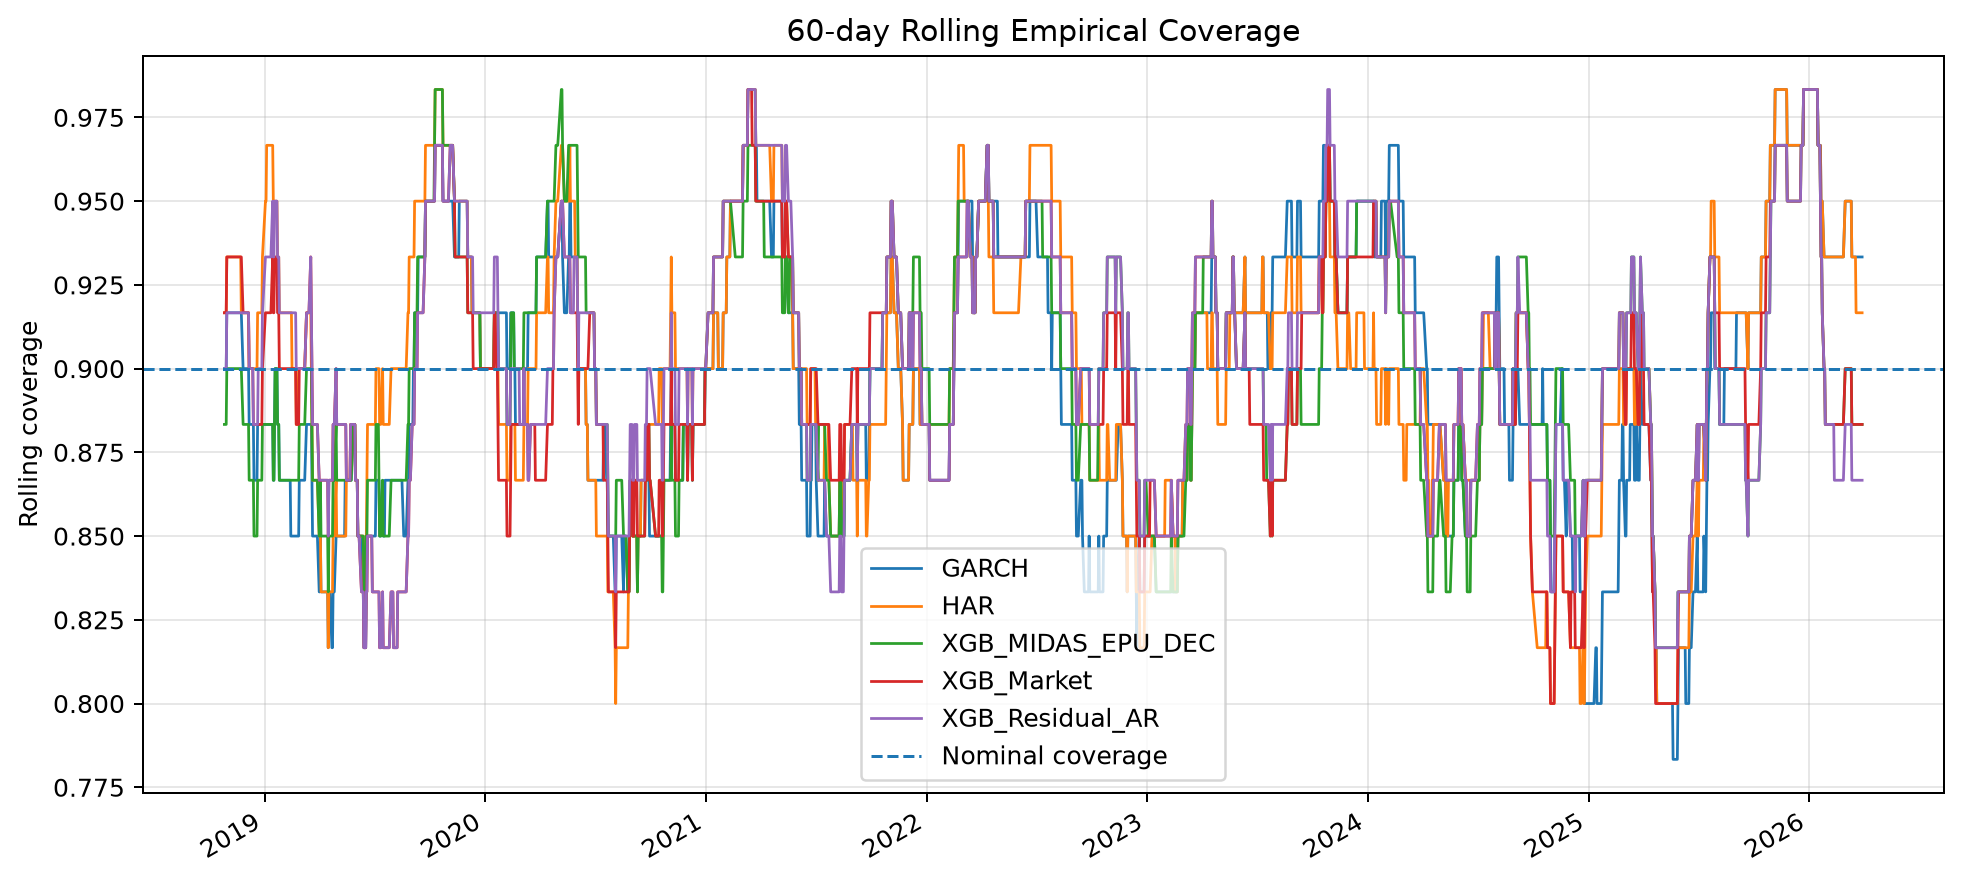
\includegraphics[width=.9\textwidth]{../../results/revised/intervals/fig_rolling_coverage_main.png}
\caption{Rolling coverage over 60 observations within the common evaluation period.}
\label{fig:rolling_coverage}
\end{figure}
\begin{figure}[htbp]\centering
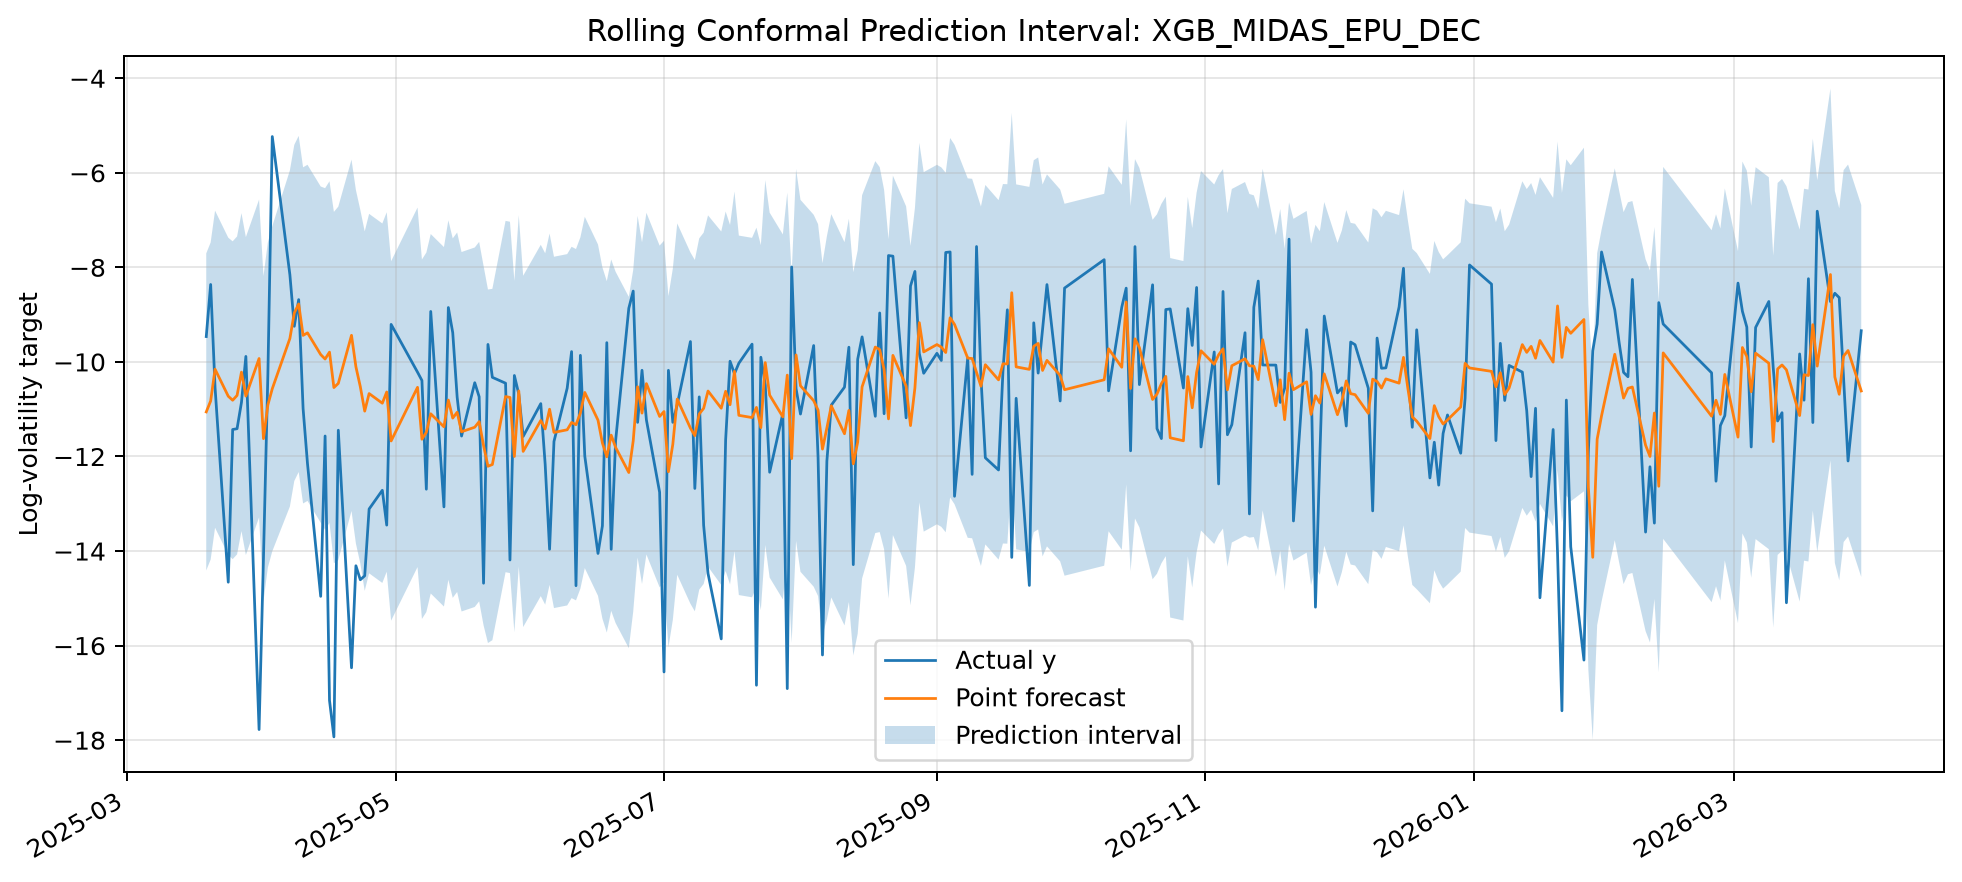
\includegraphics[width=.9\textwidth]{../../results/revised/intervals/fig_interval_series_XGB_MIDAS_EPU_DEC.png}
\caption{Recent revised DEC intervals from rolling absolute residuals.}
\label{fig:interval_series_xgb_midas}
\end{figure}

\subsection{Window sensitivity}
\begin{table}[htbp]\centering
\caption{Mean scores for 90\% intervals on the same 1859 dates.}
\label{tab:interval_robustness}
\begin{tabular}{lrrr}\toprule Model & Window 120 & Window 250 & Window 500\\\midrule
HAR & 9.7468 & 9.6973 & 9.6938\\
GARCH(1,1) & 12.6511 & 12.6634 & 12.6021\\
XGB-Market & 9.9336 & 9.8534 & 9.8528\\
XGB-AR & 9.9387 & 9.8793 & 9.8628\\
DEC & 10.2852 & 10.1995 & 10.1807\\\bottomrule
\end{tabular}
\end{table}

All 30 settings, including both nominal levels, are supplied in the accompanying results. Conclusions should be tied to the particular window and level, rather than generalized from the main setting alone. The main DEC score changes from the historical 10.1991 to 10.1995 after revision, a slight deterioration; the numerical correction does not reverse the benchmark conclusion.

For CSI300, lower QLIKE and better interval scores are distinct claims. The revised analysis does not support both simultaneously. These findings apply to the future observed proxy and this residual-based interval construction; they do not establish valid confidence intervals for latent variance.
